PHẦN I. Câu trắc nghiệm nhiều phương án lựa chọn. Thí sinh trả lời từ câu 1 đến câu 12. Mỗi câu hỏi
thí sinh chỉ chọn một phương án.
%Câu 1
\begin{ex}
	\immini{
		Cho tứ diện $ABCD$. Các vectơ có điểm đầu là $A$ và điểm cuối là các đỉnh còn lại của hình tứ diện là
		\choice
		{$\vec{AB},\vec{CA},\vec{AD}$}
		{$\vec{BA},\vec{AC},\vec{AD}$}
		{$\vec{AB},\vec{AC},\vec{DA}$}
		{\True $\vec{AB},\vec{AC},\vec{AD}$}
	}{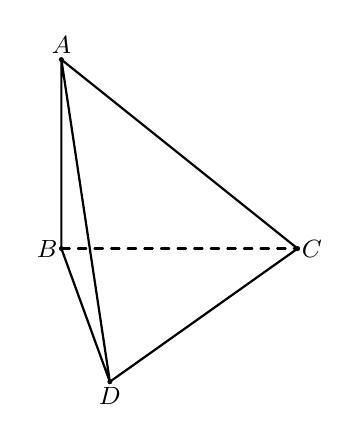
\begin{tikzpicture}[line join = round, line cap = round, thick, font = \small, scale = .6]
        \path
        (0:0) coordinate (B)
        +(0:5) coordinate (C)
        +(-70:3) coordinate (D)
        ++(90:4) coordinate (A)
        ;
        \draw[dashed]
        (B)--(C)
        ;
        \draw
        (A)--(B)--(D)--(C)--cycle
        (A)--(D)
        ;
        \foreach \x/\g in {B/180,C/0,D/-90,A/90}
        \fill (\x) circle (1.5pt)
        +(\g:3mm) node {$\x$};
    \end{tikzpicture}
	}
	\loigiai{
	}
\end{ex}
%Câu 2
\begin{ex}
	\immini{
	Cho hình lăng trụ tam giác $ABC.A'B'C'$.Gọi $M$, $N$ lần lượt là trung điểm của $AB$, $AC$. Trong 4 vectơ $\vec{AB}$, $\vec{CB}$, $\vec{B'C'}$, $\vec{A'C'}$ vectơ  nào cùng hướng với vectơ $\vec{MN}$
	\choice
	{$\vec{AB}$}
	{$\vec{CB}$}
	{\True $\vec{B'C'}$}
	{$\vec{A'C'}$}
	}{\begin{tikzpicture}[line join = round, line cap = round, thick, font = \small, scale = .7]
			\path
			(0:0) coordinate (A)
			+(0:4) coordinate (C)
			+(-50:2) coordinate (B)
			+(75:3.5) coordinate (A')
			($(A')+(B)-(A)$) coordinate (B')
			($(A')+(C)-(A)$) coordinate (C')
			($(A)!.5!(B)$) coordinate (M)
			($(A)!.5!(C)$) coordinate (N)
			;
			\draw[dashed]
			(A)--(C) (M)--(N)
			;
			\draw
			(A)--(B)--(C)--(C')--(A')--cycle
			(B')--(A') (B')--(B) (B')--(C')
			;
			\foreach \x/\g in {A/180,B/-90,C/0,A'/-180,B'/70,C'/0,M/-135,N/-45}
			\fill (\x) circle (1.5pt)
			+(\g:3mm) node {$\x$};
		\end{tikzpicture}
	}
	\loigiai{
		Vì $MN$ là đường trung bình của tam giác $ABC$ nên $MN$ song song với $BC$. Mà tứ giác $BCC'B'$ là hình bình hành. Do đó $MN$ song song với $B'C'$. Vậy hai vectơ $\vec{MN}$ và $\vec{B'C'}$ cùng hướng.
	}
\end{ex}
%Câu 3
\begin{ex}
	\immini{
		Cho hình hộp $ABCD.A'B'C'D'$.Số các vectơ có điểm đầu, điểm cuối là các đỉnh của hình hộp và bằng vectơ $\vec{AB}$ là
		\choice
		{$1$}
		{$2$}
		{\True $3$}
		{$4$}
	}{ \begin{tikzpicture}[line join = round, line cap = round, thick, font = \small, scale = .7]
			\path
			(0:0) coordinate (D')
			+(75:3.5) coordinate (D)
			+(0:3) coordinate (C')
			+(40:2) coordinate (A')
			($(C')+(D)-(D')$) coordinate (C)
			($(D)+(A')-(D')$) coordinate (A)
			($(C')+(A')-(D')$) coordinate (B')
			($(C)+(A)-(D)$) coordinate (B)
			;
			\draw[dashed]
			(A')--(A) (A')--(B') (A')--(D')
			;
			\draw
			(A)--(B)--(B')--(C')--(D')--(D)--cycle
			(C)--(B) (C)--(D) (C)--(C')
			;
			\foreach \x/\g in {D'/-90,C'/-90,D/180,A'/135,C/-45,A/90,B'/0,B/90}
			\fill (\x) circle (1.5pt)
			+(\g:3mm) node {$\x$};
		\end{tikzpicture}
	}
	\loigiai{
		$\vec{AB}=\vec{DC}=\vec{D'C'}=\vec{A'B'}$
	}
\end{ex}
%Câu 4
\begin{ex}
	Cho hình hộp $ABCD.A'B'C'D'$. Trong các khẳng định dưới đây, đâu là khẳng định đúng?
	\choice
	{$\vec{AB}+\vec{AC}+\vec{AD}=\vec{AC'}$}
	{\True $\vec{AB}+\vec{AA'}+\vec{AD}=\vec{AC'}$}
	{$\vec{AB}+\vec{AA'}+\vec{AD}=\vec{AC}$}
	{$\vec{AB}+\vec{AA'}+\vec{AD}=\vec{0}$}
	\loigiai{
		Xét hình hộp $ABCD.A'B'C'D'$ ta có $\vec{AB}+\vec{AA'}+\vec{AD}=\vec{AC'}$
	}
\end{ex}
%Câu 5
\begin{ex}
	Trong không gian cho tam giác $ABC$ có $G$ là trọng tâm và điểm $M$ nằm ngoài mặt phẳng $(ABC)$. Khẳng định nào sau đây là đúng?
	\choice
	{$\vec{MA}+\vec{MB}+\vec{MC}=\vec{0}$}
	{$\vec{GA}+\vec{GB}+\vec{GC}=0$}
	{$\vec{MA}+\vec{MB}+\vec{MC}=\vec{MG}$}
	{\True $\vec{MA}+\vec{MB}+\vec{MC}=3\vec{MG}$}
	\loigiai{
		Xét hình chóp $M \cdot ABC$ ta có: $\vec{MA}+\vec{MB}+\vec{MC}=3\vec{MG}$
	}
\end{ex}
%Câu 6
\begin{ex}
	Cho hình chóp đều $S \cdot ABCD$ tất cả các cạnh bằng $2\sqrt{3}$ (đvđd). Tính độ dài vectơ  $\vec{u}=\vec{SA}-\vec{SC}$
	\choice
	{$\sqrt{3}$}
	{$\sqrt{2}$}
	{\True $2\sqrt{6}$}
	{$2\sqrt{2}$}
	\loigiai{
		Ta có: $\left| \vec{u} \right|=\left| \vec{SA}-\vec{SC} \right|=\left| \vec{CA} \right|=2\sqrt{6}$
	}
\end{ex}
%Câu 7
\begin{ex}
	Cho tứ diện $ABCD$. Mệnh đề nào dưới đây là mệnh đề đúng?
	\choice
	{$\vec{BC}-\vec{BA}=\vec{DA}-\vec{DC}$}
	{$\vec{AC}-\vec{AD}=\vec{BD}-\vec{BC}$}
	{\True $\vec{AB}-\vec{AC}=\vec{DB}-\vec{DC}$}
	{$\vec{AB}-\vec{AD}=\vec{CD}-\vec{CB}$}
	\loigiai{
		{\centering\color{red} HINH O DAY}\\
		Ta có: $\heva{& \vec{AB}-\vec{AC}=\vec{CB} \\& \vec{DB}-\vec{DC}=\vec{CB}}\Rightarrow \vec{AB}-\vec{AC}=\vec{DB}-\vec{DC}$
	}
\end{ex}
%Câu 8
\begin{ex}
	Cho hình lăng trụ $ABC.A'B'C'$, $M$ là trung điểm của $BB'$. Đặt $\vec{CA}=\vec{a}$, $\vec{CB}=\vec{b}$, $\vec{AA'}=\vec{c}$. Khẳng định nào sau đây đúng?
	\choice
	{$\vec{AM}=\vec{b}+\vec{c}-\dfrac{1}{2}\vec{a}$}
	{$\vec{AM}=\vec{a}-\vec{c}+\dfrac{1}{2}\vec{b}$}
	{$\vec{AM}=\vec{a}+\vec{c}-\dfrac{1}{2}\vec{b}$}
	{\True $\vec{AM}=\vec{b}-\vec{a}+\dfrac{1}{2}\vec{c}$}
	\loigiai{
		{\centering\color{red} HINH O DAY}\\
		Ta có: $\vec{AM}=\vec{AB}+\vec{BM}=\vec{CB}-\vec{CA}+\dfrac{1}{2}\vec{BB'}$ $=\vec{CB}-\vec{CA}+\dfrac{1}{2}\vec{AA'}=\vec{b}-\vec{a}+\dfrac{1}{2}\vec{c}$
	}
\end{ex}
%Câu 9
\begin{ex}
	Cho hình lập phương $ABCD.A'B'C'D'$ cạnh $a$. Tính độ dài véctơ $\vec{x}=\vec{A'C'}-\vec{A'A}$ theo $a$?
	\choice
	{$a\sqrt{2}$}
	{$\dfrac{a\sqrt{3}}{2}$}
	{$a\sqrt{6}$}
	{\True $a\sqrt{3}$}
	\loigiai{
		{\centering\color{red} HINH O DAY}\\
		Ta có $\vec{x}=\vec{A'C'}-\vec{A'A}=\vec{AC'}$
	}
\end{ex}
%Câu 10
\begin{ex}
	Cho tứ diện $S \cdot ABC$ có $M$, $N,P$ là trung điểm của $SA$, $SB$, $SC$. Tìm khẳng định đúng?
	{\centering\color{red} HINH O DAY}
	\choice
	{$\vec{AB}=\dfrac{1}{2}\left(\vec{PN}-\vec{PM}\right)$}
	{$\vec{AB}=\vec{PN}-\vec{PM}$}
	{$\vec{AB}=2\left(\vec{PM}-\vec{PN}\right)$}
	{\True $\vec{AB}=2\left(\vec{PN}-\vec{PM}\right)$}
	\loigiai{
		Ta có: $\vec{AB}=2\vec{MN}=2\left(\vec{PN}-\vec{PM}\right)$
	}
\end{ex}
%Câu 11
\begin{ex}
	Cho tứ diện $S \cdot ABC$ có đáy là tam giác đều cạnh $a$, $SB$ vuông góc với đáy và $SB=\sqrt{3}a$. Góc giữa hai vectơ  $\left(\vec{AB},\vec{AS}\right)$ là
	{\centering\color{red} HINH O DAY}
	\choice
	{\True $60^\circ$}
		{$30^\circ$}
		{$45^\circ$}
		{$90^\circ$}
		\loigiai{
		Ta có: $\left(\vec{AB},\vec{AS}\right)=\widehat{SAB}$.\\
		Xét $\triangle SBA$ vuông tại $B$ ta có: $\tan \left(\widehat{SAB}\right)=\dfrac{SB}{AB}=\sqrt{3}$. Suy ra: $\left(\vec{AB},\vec{AS}\right)={{60}^\circ}$
	}
\end{ex}
%Câu 12
\begin{ex}
	Cho hình chóp $S \cdot ABC$ có $AB=4,\widehat{BAC}={{60}^\circ},\vec{AB} \cdot \vec{AC}=6$. Khi đó độ dài $\vec{AC}$ là
	\choice
	{\True $3$}
	{$6$}
	{$4$}
	{$12$}
	\loigiai{
		Ta có: $\vec{AB} \cdot \vec{AC}=AB \cdot AC \cdot \cos \widehat{BAC}$ $\Leftrightarrow 6=4 \cdot AC \cdot \cos {{60}^\circ}$ $\Leftrightarrow AC=3$.\\
		PHẦN II. Câu trắc nghiệm đúng sai. Thí sinh trả lời từ câu 1 đến câu 4. Trong mỗi ý a), b), c), d) ở mỗi\\
		câu, thí sinh chọn đúng hoặc sai
	}
\end{ex}
%Câu 13
\begin{ex}
	Cho tứ diện $ABCD$ có $AB=AC=AD=a$ và $\widehat{BAC}=\widehat{BAD}=60^\circ ,\widehat{CAD}=90^\circ $. Gọi $I$ là điểm trên cạnh $AB$ sao cho $AI=3IB$ và $J$ là trung điểm của $CD$. Gọi $\alpha $ là góc giữa hai vectơ  $\vec{AB}$ và $\vec{IJ}$.
		{\centering\color{red} HINH O DAY}
	a) Tam giác $BCD$ vuông cân
	b) $\vec{IJ}=\dfrac{1}{2}\vec{AC}+\dfrac{1}{2}\vec{AD}+\dfrac{3}{2}\vec{AB}$
	c) $\vec{AB} \cdot \vec{AC}+\vec{AC} \cdot \vec{AD}+\vec{AD} \cdot \vec{AB}=\dfrac{a^2}{2}$
	d) $\cos \alpha =-\dfrac{\sqrt{5}}{5}$
	\loigiai{
	a) (Đ). b) (S). c) (S). d) (Đ).\\
	{\centering\color{red} HINH O DAY}\\
	a) Dễ thấy tam giác $ABC$, $ABD$ đều cạnh bằng $a$, tam giác $ACD$ vuông cân đỉnh $A\Rightarrow CD=a\sqrt{2}$. Vậy tam giác $BCD$ có $BC=BD=a,CD=a\sqrt{2}$ nên tam giác $BCD$ vuông cân.\\
	b) $\vec{IJ}=\vec{IA}+\vec{AJ}=-\dfrac{3}{4}\vec{AB}+\dfrac{1}{2}\left(\vec{AC}+\vec{AD}\right)=\dfrac{1}{2}\vec{AC}+\dfrac{1}{2}\vec{AD}-\dfrac{3}{4}\vec{AB}$.\\
	c) Ta có: $\vec{AC} \cdot \vec{AD}=0$; $\vec{AB} \cdot \vec{AD}=AB \cdot AD \cdot cos60^\circ =\dfrac{a^2}{2}$; $\vec{AC} \cdot \vec{AB}=\dfrac{a^2}{2}$.\\
	$\vec{AB} \cdot \vec{AC}+\vec{AC} \cdot \vec{AD}+\vec{AD} \cdot \vec{AB}=a^2$.\\
	d) Ta có $IJ^2={{\vec{IJ}}^2}\,=\dfrac{1}{4}{{\left(\vec{AC}+\vec{AD}-\dfrac{3}{2}\vec{AB}\right)}^2}=\dfrac{1}{4}\left(\dfrac{17}{4}a^2+2\vec{AC} \cdot \vec{AD}-3\vec{AC} \cdot \vec{AB}-3\vec{AB} \cdot \vec{AD}\right)=\dfrac{5a^2}{16}\Rightarrow IJ=\dfrac{a\sqrt{5}}{4}$.\\
	$\vec{IJ}\, \cdot \vec{AB}=\dfrac{1}{2}\left(\vec{AC}+\vec{AD}-\dfrac{3}{2}\vec{AB}\right) \cdot \vec{AB}=\,\dfrac{1}{2}\left(\vec{AC} \cdot \vec{AB}+\vec{AD} \cdot \vec{AB}-\dfrac{3}{2}{{\vec{AB}}^2}\right)=-\dfrac{a^2}{4}$.\\
	$\cos \left(\vec{IJ}\,,\vec{AB}\right)=\dfrac{\vec{IJ}\, \cdot \vec{AB}}{IJ \cdot AB}=\dfrac{-\dfrac{a^2}{4}}{\dfrac{a\sqrt{5}}{4} \cdot a}=-\dfrac{\sqrt{5}}{5}$
	}
\end{ex}
%Câu 14
\begin{ex}
	Cho tứ diện $ABCD$. Gọi $M$, $N$, $P$, $Q$, $R$, $S$, $G$ lần lượt là trung điểm các đoạn thẳng $AB$, $CD$, $AC$, $BD$, $AD$, $BC$, $MN$.
		{\centering\color{red} HINH O DAY}
	a) $\vec{MR}=\vec{SN}$.
	b) $\vec{GA}+\vec{GB}+\vec{GC}+\vec{GD}=\vec{0}$.
	c) $2\vec{PQ}=\vec{AB}+\vec{AC}+\vec{AD}$.
	d) $\left| \vec{IA}+\vec{IB}+\vec{IC}+\vec{ID} \right|$ nhỏ nhất khi và chỉ khi điểm $I$ trùng với điểm $G$
	\loigiai{
	a. (Đ). b. (Đ). c. (S). d. (Đ).\\
	{\centering\color{red} HINH O DAY}\\
	a. $\left. \begin{aligned}
			& \vec{MR}=\dfrac{1}{2}\vec{BD} \\& \vec{SN}=\dfrac{1}{2}\vec{BD} \end{aligned} \right\}\Rightarrow \vec{MR}=\vec{SN}$.\\
	b. Vì $M$ là trung điểm của $AB$ nên $\vec{GA}+\vec{GB}=2\vec{GM}$\\
	Vì $N$ là trung điểm của $CD$ nên $\vec{GC}+\vec{GD}=2\vec{GN}$\\
	Vì $G$ là trung điểm của $MN$ nên $\vec{GM}+\vec{GN}=\vec{0}$\\
	Do đó: $\vec{GA}+\vec{GB}+\vec{GC}+\vec{GD}=2\left(\vec{GM}+\vec{GN}\right)=2 \cdot \vec{0}=\vec{0}$.\\
	c. $\vec{PQ}=\vec{AQ}-\vec{AP}=\dfrac{1}{2}\left(\vec{AB}+\vec{AD}\right)-\dfrac{1}{2}\vec{AC}\Leftrightarrow 2\vec{PQ}=\vec{AB}-\vec{AC}+\vec{AD}$\\
	d. Ta có:\\
	$\vec{IA}+\vec{IB}+\vec{IC}+\vec{ID}=4\vec{IG}+\left(\vec{GA}+\vec{GB}+\vec{GC}+\vec{GD}\right)=4\vec{IG}$.\\
	$\Rightarrow \left| \vec{IA}+\vec{IB}+\vec{IC}+\vec{ID} \right|=\left| 4\vec{IG} \right|=4IG$\\
	Do đó: $\left| \vec{IA}+\vec{IB}+\vec{IC}+\vec{ID} \right|$ nhỏ nhất khi $IG=0\Leftrightarrow I\equiv G$
	}
\end{ex}
%Câu 15
\begin{ex}
	Cho hình hộp chữ nhật $ABCD \cdot EFGH$ có $AB=AE=2$, $AD=3$ và đặt $\vec{a}=\vec{AB},\vec{b}=\vec{AD},\vec{c}=\vec{AE}$. Lấy điểm $M$ thỏa $\vec{AM}=\dfrac{1}{5}\vec{AD}$ và điểm $N$ thỏa $\vec{EN}=\dfrac{2}{5}\vec{EC}$. (tham khảo hình vẽ)
	{\centering\color{red} HINH O DAY}
	Khi đó ta có
	a) $\vec{MA}=-\dfrac{1}{5}\vec{b}$.
	b) $\vec{EN}=\dfrac{2}{5}\left(\vec{a}-\vec{b}+\vec{c}\right)$.
	c) ${{\left(m \cdot \vec{a}+n \cdot \vec{b}+n \cdot \vec{c}\right)}^2}=m^2 \cdot {{\vec{a}}^2}+n^2 \cdot {{\vec{b}}^2}+p^2 \cdot {{\vec{c}}^2}$ với $m,n,p$ là các số thực.
	d) $MN=\dfrac{\sqrt{61}}{5}$
	\loigiai{
	FB tác giả: Đặng Phước Thiên
	A	B	C	D
	Đúng	Sai	Đúng	Đúng
	Ta có $\vec{MA}=-\vec{AM}=-\dfrac{1}{5}\vec{AD}=-\dfrac{1}{5}\vec{b}$.\\
	$\vec{EN}=\dfrac{2}{5}\vec{EC}=\dfrac{2}{5}\left(\vec{EF}+\vec{EH}+\vec{EA}\right)=\dfrac{2}{5}\left(\vec{a}+\vec{b}-\vec{c}\right)$.\\
	${{\left(m \cdot \vec{a}+n \cdot \vec{b}+p \cdot \vec{c}\right)}^2}=m^2 \cdot {{\vec{a}}^2}+n^2 \cdot {{\vec{b}}^2}+p^2 \cdot {{\vec{c}}^2}+2mn \cdot \vec{a} \cdot \vec{b}+2np \cdot \vec{b} \cdot \vec{c}+2mp \cdot \vec{a} \cdot \vec{c}$\\
	$=m^2 \cdot {{\vec{a}}^2}+n^2 \cdot {{\vec{b}}^2}+p^2 \cdot {{\vec{c}}^2}$. (vì $\vec{a},\vec{b},\vec{c}$ đôi một vuông góc nên $\vec{a} \cdot \vec{b}=\vec{b} \cdot \vec{c}=\vec{a} \cdot \vec{c}=0$).\\
	Ta có $\vec{MN}=\vec{MA}+\vec{AE}+\vec{EN}=-\dfrac{1}{5}\vec{b}+\vec{c}+\dfrac{2}{5}\left(\vec{a}+\vec{b}-\vec{c}\right)=\dfrac{2}{5}\vec{a}+\dfrac{1}{5}\vec{b}+\dfrac{3}{5}\vec{c}$.\\
	$MN^2={{\vec{MN}}^2}={{\left(\dfrac{2}{5}\vec{a}+\dfrac{1}{5}\vec{b}+\dfrac{3}{5}\vec{c}\right)}^2}=\dfrac{4}{25}{{\vec{a}}^2}+\dfrac{1}{25}{{\vec{b}}^2}+\dfrac{9}{25}{{\vec{c}}^2}=\dfrac{4}{25} \cdot 4+\dfrac{1}{25} \cdot 9+\dfrac{9}{25} \cdot 4=\dfrac{61}{25}$.\\
	Suy ra $MN=\dfrac{\sqrt{61}}{5}$
	}
\end{ex}
%Câu 16
\begin{ex}
	Cho hình lăng trụ tam giác đều $ABC \cdot A_1B_1C_1$ có cạnh đáy bằng $x$ và chiều cao bằng $y$. (tham khảo hình vẽ)
	{\centering\color{red} HINH O DAY}
	Khi đó ta có
	a) $\vec{AB} \cdot \vec{AC}=\dfrac{1}{2}x^2$.
	b) $\vec{AC_1}=\vec{AC}+\vec{AA_1}$.
	c) $\vec{CB_1}=\vec{AB}-\vec{CA}+\vec{AA_1}$.
	d) Góc $\left(AC_1,CB_1\right)>60^\circ $ khi $\dfrac{y}{x}<\sqrt{2}$
	\loigiai{
		FB tác giả: Đặng Phước Thiên
		A	B	C	D
		Đúng	Đúng	Sai	Đúng
		Ta có $\vec{AB} \cdot \vec{AC}=AB \cdot AC \cdot \cos 60^\circ =\dfrac{1}{2}x^2$.\\
		$\vec{AC_1}=\vec{AC}+\vec{AA_1}$\\
		$ACC_1A_1$ là hình chữ nhật nên ta có $\vec{AC_1}=\vec{AC}+\vec{AA_1}$.\\
		$\vec{CB_1}=\vec{CB}+\vec{CC_1}=\vec{AB}-\vec{AC}+\vec{AA_1}$.\\
		Ta có $\vec{AC_1} \cdot \vec{CB_1}=\left(\vec{AC}+\vec{AA_1}\right) \cdot \left(\vec{AB}-\vec{AC}+\vec{AA_1}\right)=y^2-\dfrac{1}{2}x^2$ và $AC_1=CB_1=\sqrt{x^2+y^2}$.\\
		Khi đó $\cos \left(AC_1,CB_1\right)=\left| \cos \left(\vec{AC_1},\vec{CB_1}\right) \right|=\dfrac{\left| \vec{AC_1} \cdot \vec{CB_1} \right|}{AC_1 \cdot CB_1}=\dfrac{\left| y^2-\dfrac{1}{2}x^2 \right|}{x^2+y^2}$.\\
		Theo đề $\left(AC_1,CB_1\right)>60^\circ $, suy ra $\dfrac{\left| y^2-\dfrac{1}{2}x^2 \right|}{x^2+y^2}<\dfrac{1}{2}\Leftrightarrow 3y^4-6x^2y^2<0\Leftrightarrow \dfrac{y}{x}<\sqrt{2}$.\\
		PHẦN III. Câu trắc nghiệm trả lời ngắn. Thí sinh trả lời từ câu 1 đến câu 3
	}
\end{ex}
%Câu 17
\begin{ex}
	Cho hình lăng trụ $ABC.A'B'C'$. Đặt $\vec{AB}=\vec{a},\vec{AA'}=\vec{b},\vec{AC}=\vec{c}$. Ta biểu diễn $\vec{B'C}=m\vec{a}+n\vec{b}+p\vec{c}$, khi đó $m+n+p$ bằng bao nhiêu?
	{\centering\color{red} HINH O DAY}
	\loigiai{
		Trả lời: $-1$.\\
		Ta có\\
		$\vec{B'C}=\vec{B'B}+\vec{BC}$\\
		$=-\vec{BB'}+\vec{BA}+\vec{AC}=-\vec{BB'}-\vec{AB}+\vec{AC}$\\
		$=-\vec{b}-\vec{a}+\vec{c}$\\
		$\Rightarrow \vec{B'C}=-\vec{a}-\vec{b}+\vec{c}$.\\
		Suy ra $m=-1;n=-1;p=1$. Do đó $m+n+p=-1$
	}
\end{ex}
%Câu 18
\begin{ex}
	Cho tứ diện$ABCD$, gọi $I$,$J$ lần lượt là trung điểm của $AB$ và $CD$.
	1) $\vec{IJ}\,=\,\dfrac{1}{2}\left(\vec{AC}+\vec{BD}\right)$.
	2) $\vec{IJ}\,=\,\dfrac{1}{2}\left(\vec{AD}+\vec{BC}\right)$.
	3) $\vec{IJ}\,=\,\dfrac{1}{2}\left(\vec{DC}+\vec{AD}+\vec{BD}\right)$.
	4) $\vec{IJ}\,=\,\dfrac{1}{2}\left(\vec{AB}+\vec{CD}\right)$.
	Trong các đẳng thức trên có bao nhiêu đẳng thức đúng?
	\loigiai{
	Trả lời: $3$.\\
	{\centering\color{red} HINH O DAY}\\
	Ta có:\\
	1) $\vec{AC}+\vec{BD}=\vec{AI}+\vec{IJ}+\vec{JC}+\vec{BI}+\vec{IJ}+\vec{JD}=2\vec{IJ}\Rightarrow \vec{IJ}=\dfrac{1}{2}\left(\vec{AC}+\vec{BD}\right)$. Nên 1) đúng.\\
	2) $\vec{AD}+\vec{BC}=\vec{AI}+\vec{IJ}+\vec{JD}+\vec{BI}+\vec{IJ}+\vec{JC}=2\vec{IJ}\Rightarrow \vec{IJ}=\dfrac{1}{2}\left(\vec{AD}+\vec{BC}\right)$. Nên 2) đúng.\\
	3) $\vec{AC}+\vec{BD}=\vec{AI}+\vec{IJ}+\vec{JC}+\vec{BI}+\vec{IJ}+\vec{JD}=2\vec{IJ}\Rightarrow \vec{IJ}=\dfrac{1}{2}\left(\vec{AD}+\vec{DC}+\vec{BD}\right)$. Nên 3) đúng.\\
	4) $\vec{IJ}\,=\vec{IA}+\,\vec{AJ}=\,-\dfrac{1}{2}\vec{AB}\,+\dfrac{1}{2}\left(\vec{AC}\,+\,\vec{AD}\right)=\,\dfrac{1}{2}\left(\vec{BC}+\,\vec{AD}\right)=\,\dfrac{1}{2}\left(\vec{AB}+\vec{BD}+\vec{CD}+\vec{DC}+\vec{BC}\right)$ $=\,\dfrac{1}{2}\left(\vec{AB}+\vec{CD}+2\vec{BC}\right)$. Nên 4) là sai
	}
\end{ex}
%Câu 19
\begin{ex}
	Cho tứ diện đều $ABCD$ có cạnh bằng $4$. Giá trị tích vô hướng $\vec{AB}\left(\vec{AB}-\vec{CA}\right)$ bằng
	\loigiai{
	Trả lời: $24$.\\
	Ta có:\\
	$\vec{AB}\left(\vec{AB}-\vec{CA}\right)=\vec{AB} \cdot \vec{AB}+\vec{AB} \cdot \vec{AC}={{\vec{AB}}^2}+\left| \vec{AB} \right| \cdot \left| \vec{AC} \right| \cdot \cos \left(\vec{AB},\vec{AC}\right)$\\
	$=AB^2+AB \cdot AC \cdot \cos \left(\widehat{BAC}\right)=4^2+4 \cdot 4 \cdot \cos {{60}^\circ}=4^2+\dfrac{4^2}{2}=\dfrac{{{3 \cdot 4}^2}}{2}=24$
	}
\end{ex}
%Câu 20
\begin{ex}
	Trong không gian, cho hai vectơ  $\vec{a}$ và $\vec{b}$ có cùng độ dài bằng $6$. Biết độ dài của vectơ  $\vec{a}+2\vec{b}$ bằng $6\sqrt{3}$. Biết số đo góc giữa hai vectơ  $\vec{a}$ và $\vec{b}$ là $x$ độ. Giá trị của $x$ là bao nhiêu?
	\loigiai{
	Trả lời: $120$.\\
	Ta có $6\sqrt{3}=\left| \vec{a}+2\vec{b} \right|\Leftrightarrow {{\left(6\sqrt{3}\right)}^2}={{\left| \vec{a}+2\vec{b} \right|}^2}={{\left(\vec{a}+2\vec{b}\right)}^2}$\\
	$\Leftrightarrow a^2+4b^2+4\vec{a} \cdot \vec{b}=108\Leftrightarrow 6^2+{{4 \cdot 6}^2}+4 \cdot \vec{a} \cdot \vec{b}=108\Leftrightarrow 4 \cdot \vec{a} \cdot \vec{b}=-72\Leftrightarrow \vec{a} \cdot \vec{b}=-18$.\\
	Lại có $\vec{a} \cdot \vec{b}=\left| \vec{a} \right| \cdot \left| \vec{b} \right| \cdot \cos \left(\vec{a}\,,\vec{b}\right)\Leftrightarrow \cos \left(\vec{a}\,,\vec{b}\right)=\dfrac{\vec{a} \cdot \vec{b}}{\left| \vec{a} \right| \cdot \left| \vec{b} \right|}=\dfrac{-18}{6 \cdot 6}=\dfrac{-1}{2}\Leftrightarrow \left(\vec{a}\,,\vec{b}\right)=120^\circ $.\\
	Khi đó góc giữa hai vectơ  $\vec{a}$ và $\vec{b}$ là $120^\circ $
	}
\end{ex}
%Câu 21
\begin{ex}
	Cho tứ diện đều $ABCD$ có cạnh bằng $15$. Biết độ dài của $\vec{AB}+\vec{AC}+\vec{AD}$ bằng $a\sqrt{6}$, khi đó giá trị của $a$ là?
	\loigiai{
	Trả lời: $15$.\\
	{\centering\color{red} HINH O DAY}\\
	Gọi $G$ là trọng tâm tâm giác $BCD$, $M$ là trung điểm $CD$.\\
	Ta có $\vec{GB}+\vec{GC}+\vec{GD}=\vec{0}\Leftrightarrow \left(\vec{GA}+\vec{AB}\right)+\left(\vec{GA}+\vec{AC}\right)+\left(\vec{GA}+\vec{AD}\right)=\vec{0}\Leftrightarrow 3\vec{GA}+\left(\vec{AB}+\vec{AC}+\vec{AD}\right)=\vec{0}$\\
	$\Leftrightarrow \vec{AB}+\vec{AC}+\vec{AD}=-3\vec{GA}=3\vec{AG}\Rightarrow \left| \vec{AB}+\vec{AC}+\vec{AD} \right|=\left| 3\vec{AG} \right|=3AG$.\\
	Xét tam giác đều $BCD$ có $BM=BC \cdot \dfrac{\sqrt{3}}{2}=\dfrac{15\sqrt{3}}{2}\Rightarrow BG=\dfrac{2}{3}BM=5\sqrt{3}$.\\
	Vì tứ diện $ABCD$ đều nên $AG\bot (BCD)\Rightarrow \widehat{AGB}=90^\circ $.\\
	Xét tam giác $ABG$ có $AG=\sqrt{AB^2-BG^2}=\sqrt{{{15}^2}-{{\left(5\sqrt{3}\right)}^2}}=5\sqrt{6}$.\\
	Do đó $\left| \vec{AB}+\vec{AC}+\vec{AD} \right|=3AG=15\sqrt{6}\Rightarrow a=15$.\\
	Vậy giá trị của $a=15$
	}
\end{ex}
%Câu 22
\begin{ex}
	Một chiếc cân đòn tay đang cân một vật có khối lượng $m=3\,\text{kg}$ được thiết kế với đĩa cân được giữ bởi bốn đoạn xích $SA\,,SB\,,SC\,,SD$ sao cho $S \cdot ABCD$ là hình chóp tứ giác đều có $\widehat{ASC}=90^\circ $. Biết độ lớn của lực căng cho mỗi sợi xích có dạng $\dfrac{a\sqrt{2}}{4}$. Lấy $g=10\,\text{m/}{{\text{s}}^{\text{2}}}$, khi đó giá trị của $a$ bằng bao nhiêu?
	{\centering\color{red} HINH O DAY}
	\loigiai{
	Trả lời: $30$.\\
	{\centering\color{red} HINH O DAY}\\
	Gọi $O$ là tâm của hình vuông $ABCD$.\\
	Ta có $\vec{\text{O}A}+\vec{OB}+\vec{OC}+\vec{OD}=\vec{0}\Leftrightarrow \vec{O\,S}+\vec{SA}+\vec{OS}+\vec{SB}+\vec{OS}+\vec{SC}+\vec{OS}+\vec{SD}=\vec{0}$\\
	$\Leftrightarrow \vec{SA}+\vec{SB}+\vec{SC}+\vec{SD}=-4\vec{OS}=4\vec{SO}\Rightarrow \left| \vec{SA}+\vec{SB}+\vec{SC}+\vec{SD} \right|=\left| 4\vec{SO} \right|=4SO$.\\
	Trọng lượng của vật nặng là $P=mg=3 \cdot 10=30\,(N)$. Suy ra $4\left| \vec{SO} \right|=P=30\,(N)\Rightarrow SO=\dfrac{15}{2}$.\\
	Lại có tam giác $ASC$ vuông cân tại $S$ nên\\
	$SO=SA \cdot \sin \widehat{SAC}\Rightarrow SA=\dfrac{SO}{\sin \widehat{SAC}}=\dfrac{\dfrac{15}{2}}{\sin 45^\circ }=\dfrac{15\sqrt{2}}{2}=\dfrac{30\sqrt{2}}{4}\Rightarrow a=30$.\\
	Vậy $a=30$
	}
\end{ex}
